



\documentclass[10pt,
 article,
 amsmath,amssymb
]{revtex4-2}



\usepackage[utf8x]{inputenc}

\usepackage[T1]{fontenc}
\usepackage{listings}
\usepackage{physics}
\usepackage{amsthm}
\usepackage{amssymb}
\usepackage{graphicx}
\usepackage[a4paper,
            bindingoffset=0.2in,
            left=1in,
            right=1in,
            top=1in,
            bottom=1in,
            footskip=.25in]{geometry}

\graphicspath{{../../../images/}}




\newtheorem{theorem}{Theorem}[section]
\newtheorem{example}[theorem]{Example}
\newtheorem{remark}[theorem]{Remark}



\newtheorem{proposition}{Proposition}
\newtheorem{corollary}{Corollary}[theorem]
\newtheorem{lemma}[theorem]{Lemma}
\newtheorem{definition}{Definition}


\newcommand{\CC}{\mathbb{C}}
\newcommand{\RR}{\mathbb{R}}
\newcommand{\LL}{\mathcal{L}}



\usepackage{tikz}

\usepackage{hyperref}


\usepackage[english]{babel}
\usepackage[english]{isodate}









\setcounter{footnote}{0}

\hypersetup{colorlinks=true,urlcolor=blue}









\begin{document}


\title{2d CFTs}



\author{Rafael C.}




\date{2025-03-21}







\maketitle

\tableofcontents



\subsection{CFTs in general dimension}


\section{2d CFTs}

Virasoro algebra.

We can define 2d CFTs on any Riemann surface. Due to Moore and Seiberg it's enough to demand consistency on sphere (genus $0$) and torus (genus $1$).

\subsection{Weyl anomaly}

\section{Bootstrap}
\begin{itemize}
    \item     State-operator correspondance $\leftrightarrow$ radial quantization
    \item Primaries: $$\mathcal{O}\to \Omega(x)^{-\Delta} \mathcal{O}(x')$$ it follows
\end{itemize}
$$\langle \mathcal{O}_1 \mathcal{O}_2\dots \mathcal{O}_n \rangle_g =\prod_{i}^{n} \Omega(x)^{-\Delta_i} \langle \mathcal{O}_1' \mathcal{O}_2'\dots \mathcal{O}_n' \rangle_{g'=\Omega(x)^2 g}$$
\begin{itemize}
    \item $1,\, 2$ and $3$ point functions fixed by conf. Symmetry (up to constant) and one point vanishing.
\end{itemize}

\section{Representations}
Irreducible representations dont have null vectors. Construct them by quotient. 
\begin{example}
    Start with some dimension
\end{example}




\section{String theory (Gaiotto)}
Point particle amplitudes: 
$$ A_\Gamma= \underbrace{\int d\ell}_{\text{Moduli}} \int_{X:\Gamma \to \RR} \mathcal{D} X e^{-S[X,\ell]}$$
\begin{itemize}
    \item Bad for regularization (singularities in vertex)
\end{itemize}
Schematically:
\begin{align*}
    A_\Gamma&= \int \prod_{(a,b)= \text{internal lines}} d p_{ab} \prod_{a=\text{internal vertices}} \prod_{(a,b)= \text{internal lines}} \frac{1}{p^2_{ab}+m^2}\\
  \frac{1}{p_{ab}^2+m^2}&=\int^\infty_0 d\ell_{ab} e^{-\ell_{ab}p_{ab}^2-\ell_{ab}m^2}\\
    \delta(\sum_b p_{ab})&=\int dx_a^d e^{i x_a \sum p_{ab}}\\
    A_\Gamma&=\prod_{a=\text{internal vertices}} \int d X_a^D e^{i X_a} \sum_{b=\text{external}}p_{ab} \prod_{(a,b)} G(x_a,x_b) \\
    G(x_a,x_b)&=\int_0^\infty d\ell_{ab} e^{\frac{(x_a-x_b)^2}{4 \ell_{ab}}-\ell_{ab}m^2}
\end{align*}
We will see how the delta conservation arrises from the non oscilatorry part of the path integral, the vertex operators insertion and the 
Strings:
$$ A_\Gamma= \underbrace{\int d\ell}_{\text{Moduli}} \int_{X:\Gamma \to \RR} \mathcal{D} X e^{-S[X,\ell]}$$


\begin{example}[Klein-Gordon propagator from the worldline (path integral)]

Consider the action for a relativistic particle propagating between two points
$$S=\frac{1}{2}\int_0^1d\tau\left[e^{-1}\dot{X}^\mu\dot{X}_\mu+m^2e\right]\quad(\dot{X}\equiv\partial_\tau X\:,\quad\mu=1,\ldots,D)\:,$$
with Dirichlet boundary conditions $X(0)=x_0$ and $X(1)=x_1.$ Here we have Wick rotated to a
Euclidean worldline and a Euclidean $D$-dimensional target space. We proceed to show how the path integral formalism allow us to compute scattering amplitudes in the point particle and string cases.


Our starting point is the following formal expression for the path integral:
$$Z(X_0,X_1)=\int_{X(0)=X_0}\frac{[dXde]}{V_{\mathrm{diff}}}\exp\left(-S_{\mathrm{m}}[X,e]\right),$$
where the action for the“matter” fields $X^\mu$ is
$$S_\text{m}[X,e]=\dfrac{1}{2}\int_0^1d\tau\:e\begin{pmatrix}e^{-1}\partial X^\mu e^{-1}\partial X_\mu+m^2\end{pmatrix}$$
(where $\partial\equiv d/d\tau).$ We have fixed the coordinate range for $\tau$ to be [0,1]. 

This action has invariance under diffeomorphisms
$\zeta:[0,1]\to[0,1]$, under which the $X^\mu$ are scalars,
$$X^{\mu\zeta}(\tau^\zeta)=X^\mu(\tau),$$
and the einbein $e$ is a“co-vector,”
$$e^\zeta(\tau^\zeta)=e(\tau)\frac{d\tau}{d\tau^\zeta}.$$ 
Think of this setup as 1d geometry with 1d metric $h_{\tau\tau}=m^2e^2.$ So the question is: how
much can you fix using co-ordinate transformations in 1d geometry?
Answer: There is no local geometry in 1d-all metrics are locally related by co-ordinate transformations. 
The only geometry can come from global features, and in 1d the only global feature is periodicity. 
The space can be either a circle or a line. If it is a circle, 
then the circumference $2\pi R=T=\int d\tau e(\tau)$ is the only diffeomorphism-invariant quantity.


Therefore, as usual, $V_\mathrm{diff}$ is the volume of this group of diffeomorphisms to which we should gauge fix and the $e$ integral
in the partition function runs over positive functions on $[0,1]$, and the integral
$$l\equiv\int_0^1d\tau\:e$$
is diffeomorphism invariant and therefore a modulus; the moduli space is $(0,\infty).$


In order to make sense of the functional integrals of $X$ we will need to define an inner 
product on the space of functions on $[0,1]$, which will induce measures on the relevant 
function spaces. This inner product will depend on the einbein $e$ in a way that is
 uniquely determined by the following two constraints:
 \begin{enumerate}
    \item the inner product must be 
    diffeomorphism invariant; 
    \item it must depend on $e(\tau)$ only locally, in other words,
     it must be of the form $$(f,g)_e=\int_0^1d\tau\:h(e(\tau))f(\tau)g(\tau),$$ for some function $h.$ 
 \end{enumerate}

As we will see, these conditions will be necessary to allow us to regularize the infnite 
products that will arise in carrying out the functional integrals in (1), and then to
 renormalize them by introducing a counter-term action, in a way that respects the symmetries
  of the action (2). For $f$ and $g$ scalars, the inner product satisfying these two 
  conditions is
$$(f,g)_e\equiv\int_0^1d\tau\:efg.$$
We can express the matter action using this inner product:
$$S_\mathrm{m}[X,e]=\frac{1}{2}(e^{-1}\partial X^\mu,e^{-1}\partial X_\mu)_e+\frac{lm^2}{2}.$$

We now wish to express the path integral of the partition function in a slightly less 
formal way by choosing a fiducial einbein $e_l$ for each point $l$ in the moduli space,
 and replacing the integral over einbeins by an integral over the moduli space times a 
 Faddeev-Popov determinant $\Delta_\mathrm{FP}[e_l].$ 
 
 Defining $\Delta_\mathrm{FP}$ by
$$1=\Delta_{\mathrm{FP}}[e]\int_0^\infty dl\int[d\zeta]\:\delta[e-e_l^\zeta],$$
we indeed have, by the usual sequence of formal manipulations
$$Z(X_0,X_1)=\int_0^\infty dl\int_{X(0)=X_0}[dX]\Delta_{\mathrm{FP}}[e_l]\exp\left(-S_{\mathrm{m}}[X,e_l]\right).$$

To calculate the Faddeev-Popov determinant at the point $e=e_l$, we expand $e$ about $e_l$ 
for small
diffeomorphisms $\zeta$ and small changes in the modulus:
$$e_l-e_{l+\delta l}^\zeta=\partial\gamma-\frac{de_l}{dl}\delta l,$$
where $\gamma$ is a scalar function parametrizing small diffeomorphisms:
 $\tau^\zeta=\tau+e^{-1}\gamma;$ to respect the fixed coordinate range,
  $\gamma$ must vanish at $0$ and $1$. Since the variation of $e$ is, like $e$, a co-vector,
   we will for simplicity multiply it by $e_l^{-1}$ in order to have a scalar,
    and then bring into play our innen product (7) in order to express the delta 
    functional in (9) as an integral over scalar functions $\beta:$
$$\Delta_{\mathrm{FP}}^{-1}[e_l]=\int d\delta l[d\gamma d\beta]\:\exp\left(2\pi i(\beta,e_l^{-1}\partial\gamma-e_l^{-1}\frac{de_l}{dl}\delta l)_{e_l}\right)$$

The integral is inverted by replacing the bosonic variables $\delta l,\gamma$, and $\beta$ by Grassman variables $\xi,c$,
and $b{:}$
$$\begin{aligned}\Delta_{\mathrm{FP}}[e_{l}]&=\int d\xi[dcdb]\:\exp\left(\frac1{4\pi}(b,e_l^{-1}\partial c-e_l^{-1}\frac{de_l}{dl}\xi)_{e_l}\right)\\&=\int[dcdb]\:\frac1{4\pi}(b,e_l^{-1}\frac{de_l}{dl})_{e_l}\exp\left(\frac1{4\pi}(b,e_l^{-1}\partial c)_{e_l}\right).\end{aligned}$$

We can now write the path integral in a more explicit form:
$$\begin{aligned}Z(X_{0},X_{1})&=\int_0^\infty dl\int_{X(0)=X_0}[dX]\int_{c(0)=c(1)=0}[dcdb]\:\frac1{4\pi}(b,e_l^{-1}\frac{de_l}{dl})_{e_l}\\&\times\exp\left(-S_{\mathrm{g}}[b,c,e_l]-S_{\mathrm{m}}[X,e_l]\right),\end{aligned}$$
where
$$S_\text{g}[b,c,e_l]=-\frac{1}{4\pi}(b,e_l^{-1}\partial c)_{e_l}.$$

At this point it becomes convenient to work in a specific gauge, the simplest being
$$e_l(\tau)=l.$$
Then the inner product becomes simply
$$(f,g)_l=l\int_0^1d\tau\:fg.$$
In order to evaluate the Faddeev-Popov determinant, let us decompose $b$ and $c$ into nor-
malized eigenfunctions of the operator
$$\Delta=-(e_l^{-1}\partial)^2=-l^{-2}\partial^2:$$
$$\begin{aligned}&b(\tau)=\:\frac{b_{0}}{\sqrt{l}}+\sqrt{\frac{2}{l}}\sum_{j=1}^{\infty}b_{j}\cos(\pi j\tau),\\&c(\tau)=\sqrt{\frac{2}{l}}\sum_{j=1}^{\infty}c_{j}\sin(\pi j\tau),\end{aligned}$$
with eigenvalues
$$\nu_j=\frac{\pi^2j^2}{l^2}.$$
The ghost action becomes
$$S_{\mathrm{g}}(b_j,c_j,l)=-\frac{1}{4l}\sum_{j=1}^{\infty}jb_jc_j.$$

The zero mode $b_0$ does not enter into the action, but it is singled out by the
 insertion appearing in
front of the exponential in the Fadeev-Popov determinant:
$$\frac1{4\pi}(b,e_l^{-1}\frac{de_l}{dl})_{e_l}=\frac{b_0}{4\pi\sqrt{l}}.$$


The Faddeev-Popov determinant is, finally,
$$\begin{aligned}\Delta_{\mathrm{FP}}(l)&=\int\prod_{j=0}^\infty db_j\prod_{j=1}^\infty dc_j\frac{b_0}{4\pi\sqrt{l}}\exp\left(\frac1{4l}\sum_{j=1}^\infty jb_jc_j\right)\\&=\frac1{4\pi\sqrt{l}}\prod_{j=1}^\infty\frac j{4l}\\&=\frac1{4\pi\sqrt{l}}\mathrm{det}^{\prime}\left(\frac\Delta{16\pi^2}\right)^{1/2},\end{aligned}$$
the prime on the determinant denoting omission of the zero eigenvalue.


Let us decompose $X^\mu(\tau)$ into a part which obeys the classical equations of motion,
$$X_{\mathrm{cl}}^\mu(\tau)=X_0+(X_1-X_0)\tau,$$
plus quantum fuctuations; the fluctuations vanish at $0$ and $1$, and can therefore be decomposed
into the same normalized eigenfunctions of $\Delta$ as $c$ was:
$$X^\mu(\tau)=X_{\text{cl}}^\mu(\tau)+\sqrt{\frac{2}{l}}\sum_{j=1}^\infty x_j^\mu\sin(\pi j\tau).$$
The matter action becomes
$$S_\text{m}(X_0,X_1,x_j)=\frac{(X_1-X_0)^2}{2l}+\frac{\pi^2}{l^2}\sum_{j=1}^\infty j^2x_j^2+\frac{lm^2}{2},$$
and the matter part of the path integral
$$\begin{aligned}\int_{X(0)=X_0}[dX]\:\exp\left(-S_\mathrm{m}[X,e_l]\right)&=\exp\left(-\frac{(X_1-X_0)^2}{2l}-\frac{lm^2}2\right)\int\prod_{\mu=1}^D\prod_{j=1}^\infty dx_j^\mu\exp\left(-\frac{\pi^2}{l^2}\sum_{j=1}^\infty j^2x_j^2\right)\\&=\exp\left(-\frac{(X_1-X_0)^2}{2l}-\frac{lm^2}2\right)\det^{\prime}\left(\frac\Delta\pi\right)^{-D/2},\end{aligned}$$
where we have conveniently chosen to work in a Euclidean spacetime in order to make all of the
Gaussian integrals convergent.

Putting together the results, and dropping the irrelevant constant factors
multiplying the operator $\Delta$ in the infnite-dimensional determinants, we have:
$$Z(X_0,X_1)=\int_0^\infty dl\:\frac{1}{4\pi\sqrt{l}}\exp\left(-\frac{(X_1-X_0)^2}{2l}-\frac{lm^2}{2}\right)\left(\det'\Delta\right)^{(1-D)/2}.$$

We will regularize the determinant of $\Delta$ in the same way as it is done in Appendix A.1 of Polchinski, by dividing
by the determinant of the operator $\Delta+\Omega^2$:
$$\begin{aligned}\frac{\mathrm{det'}\Delta}{\mathrm{det'}(\Delta+\Omega^2)}&=\prod_{j=1}^\infty\frac{\pi^2j^2}{\pi^2j^2+\Omega^2l^2}\\&=\frac{\Omega l}{\sinh\Omega l}\\&\sim2\Omega l\exp\left(-\Omega l\right),\end{aligned}$$
where the last line is the asymptotic expansion for large $\Omega.$ The path integral becomes
$$\begin{aligned}&Z(X_0,X_1)\\&=\frac1{4\pi(2\Omega)^{(D-1)/2}}\int_0^\infty dl\:l^{-D/2}\exp\left(-\frac{(X_1-X_0)^2}{2l}-\frac{l(m^2-(D-1)\Omega)}2\right).\end{aligned}$$


The inverse divergence due to the factor of $\Omega^{(1-D)/2}$ in front of the integral can be dealt with by a field renormalization, but since we will not concern ourselves with the overall normalization of the path integral we will simply drop all of the factors that appear in front. The divergence coming from the $\Omega$ term in the exponent can be cancelled by a (diffeomorphism invariant) counterterm in the action,
$$S_{\mathrm{ct}}=\int_0^1d\tau\:eA=lA$$
The mass $m$ is renormalized by what is left over after the cancellation of infinities,
$$m_{\mathrm{phys}}^2=m^2-(D-1)\Omega-2A,$$
but for simplicity we will assume that a renormalization condition has been chosen that sets $m_\mathrm{phys}=m.$

We can now proceed to the integration over moduli space:
$$Z(X_0,X_1)=\int_0^\infty dl\:l^{-D/2}\exp\left(-\frac{(X_1-X_0)^2}{2l}-\frac{lm^2}{2}\right).$$
The integral is most easily done after passing to momentum space:
$$\begin{aligned}\tilde{Z}(k)&\equiv\int d^DX\:\exp\left(ik\cdot X\right)Z(0,X)\\&=\int_0^\infty dl\:l^{-D/2}\exp\left(-\frac{lm^2}2\right)\int d^DX\:\exp\left(ik\cdot X-\frac{X^2}{2l}\right)\\&=\left(\frac\pi2\right)^{D/2}\int_0^\infty dl\:\exp\left(-\frac{l(k^2+m^2)}2\right)\\&=\left(\frac\pi2\right)^{D/2}\frac2{k^2+m^2};\end{aligned}$$
neglecting the constant factors, this is precisely the momentum space scalar propagator.

\end{example}
\begin{example}
    Second way of deriving the propagator. Consider the action for a relativistic particle propagating between two points

$$S=\frac{1}{2}\int_0^1d\tau\left[e^{-1}\dot{X}^\mu\dot{X}_\mu+m^2e\right]\quad(\dot{X}\equiv\partial_\tau X\:,\quad\mu=1,\ldots,D)\:,$$

(1)


with Dirichlet boundary conditions $X(0)=x_0$ and $X(1)=x_1.$ Here we have Wick rotated to a

Euclidean worldline and a Euclidean $D$-dimensional target space.

(a) Gauge symmetry. Show that this theory is invariant under 1d diffeomorphisms $\tau\to\hat{\tau}(\tau).$

How does $e$ transform?

(b) Gauge fixing. Explain why one can fıx the gauge $e(\tau)=T$ where $T:=\int d\tau e(\tau)$, and why

there is no remaining gauge symmetry.

(c) Path integral. You may assume that the correct path integral measure is $\frac{\mathcal{D}e}{\mathrm{gauge}}=dT$ afte

gauge fixing.

Expanding near the classical trajectory,

$$X=\bar{X}+\eta\:,\quad\bar{X}=x_0+\tau(x_1-x_0)\:,$$

(2)

and integrating over the fluctuation $\eta$, the propagator from $X_1$ to $X_2$ is given by the path

integral

$$G(x_0,x_1)=\int_0^\infty dT\int\mathcal{D}\eta^\mu\exp\left(-\frac12\int_0^1d\tau\left[T^{-1}\dot{X}^\mu\dot{X}_\mu+m^2T\right]\right)\:.$$

. (3)

Do the Gaussian integral over $\eta$, with boundary conditions $\eta(0)=\eta(1)=0$, to obtain

$$G(x_0,x_1)=\int_0^\infty dT\:\exp\left[-\frac12T^{-1}(x_0-x_1)^2-\frac12m^2T\right]\:\det^{\prime}\left(-\frac1{T^2}\partial_\tau^2\right)^{-D/2}.$$

(4)

[You may assume that $\int\mathcal{D}\phi e^-\frac T2\int_0^1d\tau\phi{\mathcal{O}}\phi=(\det^{\prime}\mathcal{O})^{-1/2}$ for a scalar feld $\phi.]$

(d) Functional determinant. By finding the eigenvalues of the operator $-\frac1{T^2}\partial_\tau^2$ on the ap-

propriate space of functions, evaluate this determinant to obtain

$$G(x_0,x_1)\sim\int_0^\infty dT\:\exp{[-\frac12T^{-1}(x_0-x_1)^2-\frac12m^2T]}\:\prod_{n=1}^\infty\left(\frac{\pi^2n^2}{T^2}\right)^{-D/2}\:,$$
where the overall numerical factor may be ignored.
[Hint: the symbol det' means not to include the eigenvalue 0.]

(e) Zeta-function regularization. Using the fact that $\zeta(0)=-\frac12$, and the series expansion

$\zeta(s)=\sum_{n=1}^\infty n^{-s}$ of the Riemann zeta function, evaluate this product to give

$$G(x_0,x_1)\sim\int dT\exp\left[-\frac12T^{-1}(x_0-x_1)^2-\frac12m^2T\right]T^{-D/2}\:.$$

(5)

( f) Momentum space. Take the Fourier transform to obtain the momentum- space propagator
that you already know for Klein-Gordon theory, $S=\int d^Dx\left(\partial_\mu\phi\right)^2.$

$\textit{Solution. }$

(a) Under a general diffeomorphism we have

$$\begin{aligned}&\tau\to\hat{\tau}(\tau)\:,\quad d\tau\to d\hat{\tau}=\hat{\tau}^{\prime}(\tau)d\tau\:,\\&X(\tau)\to\hat{X}(\hat{\tau})=X(\tau)\:,\quad\partial_{\tau}\to\partial_{\hat{\tau}}=\partial_{\tau}/\hat{\tau}^{\prime}(\tau)\\&e(\tau)\to\hat{e}(\hat{\tau})=e(\tau)/\hat{\tau}^{\prime}(\tau)\:.\end{aligned}$$

(6)

Everything transforms covariantly and it is easy to check that each term in the action is

invariant. 
(b) Think of this setup as 1d geometry with 1d metric $h_\tau\tau=m^2e^2.$ So the question is: how
much can you fix using co-ordinate transformations in 1d geometry?
Answer: There is no local geometry in 1d-all metrics are locally related by co-ordinate transformations. The only geometry can come from global features, and in 1d the only global feature is periodicity. The space can be either a circle or a line. If it is a circle, then the circumference $2\pi R=T=\int d\tau e(\tau)$ is the only diffeomorphism-invariant quantity.
( c) $\bullet$ Why do we gauge fix? Because one should reduce to the physical degrees of freedom
before quantizing.
$\bullet$ Why is it a non-trivial fact that $\frac{\mathcal{D}e}{\mathrm{gauge}}=dT?$ Because, in general, one should expect a $\begin{aligned}\text{non-trivial determinant }\mathcal{D}e=\mathcal{D}(\mathrm{gauge})dT\left.f(T),\mathrm{~i.e.~}\frac{\mathcal{D}e}{\mathrm{gauge}}\right.=dTf(T)\\\text{non-trivial determinant }\mathcal{D}e=\mathcal{D}(\mathrm{gauge})dT\left.f(T),\mathrm{~i.e.~}\frac{\mathcal{D}e}{\mathrm{gauge}}\right.=dTf(T)\\\text{corresponding to}\end{aligned}$ the correct gauge-invariant measure in the space of felds $e.$ In this case $f(T)=1.$
Substituting the expansion (2) into the gauge-fixed action gives
$$S=\frac12\int_0^1d\tau\big[T^{-1}(x_0-x_1)^2+m^2T+T^{-1}\dot{\eta}^2\big]\:,$$

(7)

where we dropped a cross-term $(x_0-x_1)\dot{\eta}$ since it is a total derivative
The $\eta$-dependent part of the path-integral (3) is then

$$\int\mathcal{D}\eta\exp\left(-\frac T2\int_0^1d\tau\:\eta[-\frac1{T^2}\partial_\tau^2]\eta\right)=\det^{\prime}\left(-\frac1{T^2}\partial_\tau^2\right)^{-D/2}.$$

(8)

$\bullet$ Note the measure $\int\mathcal{D}\phi\exp\left(-\frac12\int_0^1d\tau e\phi\mathcal{O}\phi\right)=\int\mathcal{D}\phi\exp\left(-\frac T2\int_0^1d\tau\phi\mathcal{O}\phi\right)$, withthe factor of $T$, is the natural diffeomorphism- invariant one. 

(d) det'$\mathcal{O}$ is just the product of the non-zero eigenvalues of $\mathcal{O}$ in the appropriate space of
functions, in this case those vanishing at 0 and 1. The eigenfunctions of $-\frac1{T^2}\partial_\tau^2$ in this space are the classical solution $\bar{x}$ and $\sin(n\pi\tau)$ with $n\in\mathbb{Z}_>0.$ The eigenvalues are 0 and $n^2\pi^2/T^2$ We remove 0 and take the product of the others.

(e) Evaluate

$$\begin{aligned}\prod_{n=1}^\infty\left(\frac{\pi^2n^2}{T^2}\right)^{-D/2}&=\text{ (const)}\prod_{n=1}^\infty T^D\\&\sim\exp\log\prod T^D\\&=\exp((\log T^D)\sum1)\\&=\exp(\zeta(0)\log T^D)\\&=\exp(-\frac12\log T^D)\\&=T^{-D/2}\:.\end{aligned}$$

( f)  We simply use

$$\int\mathrm{d}^Dx\:e^{ip\cdot x}e^{-\frac{x^2}{2T}}=(2\pi T)^{\frac D2}e^{-\frac T2p^2}$$

(9)

To get

$$G(p)=\int\mathrm{d}^Dxe^{ip\cdot x}G(x,0)\propto\int_0^\infty\mathrm{d}T\:e^{-\frac T2(p^2+m^2)}\propto\frac1{p^2+m^2}$$

(10)

Scattering amplitudes from the worldline (canonical quantization).
Consider the action for a relativistic point particle on an open path in $D$-dimensional Minkowski
space,

(11)

$$S[e,X]=\frac{1}{2}\int_{-\infty}^{\infty}d\tau\left[e^{-1}\dot{X}^{2}-m^{2}e\right]\:.$$

(a) Constraint. Write down the equation of motion from varying $e.$ Show that it is equivalent
to the vanishing of the Hamiltonian,

(12)

$$\mathcal{H}=\frac12[e^{-1}\dot{X}^2+m^2e]=0\:.$$

Since $e$ is an auxiliary field (it has no derivatives), this equation will be imposed as a
constraint on physical states, $\begin{aligned}\text{A}|\psi\rangle=0.\end{aligned}$
(b) Vertex operators. Show that the‘vertex operators’,


(13)

$$V(k)=\int d\tau\:e(\tau)\:\exp\left[ik\cdot X(\tau)\right]\:,$$

are diffeomorphism-invariant for any momentum vector $k.$
(c) Quantization. Explain why we can gauge-fix $e(\tau)=1/m$ on the infinite line (with freedom
$\dot{\text{to choose the coefficient }1}).$ In this gauge the canonical momentum is $\mathcal{P}=m\dot{X}.$
(i) Convince yourself that the Schrodinger equation gives the time evolution
$$X(\tau)=x+\tau\:\frac{1}{m}\:p\:,\quad\mathcal{P}(\tau)=p\:.$$
(14)


We impose the canonical commutation relation $[x^\mu,p^\nu]=i\eta^{\mu\nu}.$
(ii) Show, in this gauge, that $V(k)$ carries momentum $k^\mu$,
$$[p^\mu,V(k)]=k^\mu V(k)\:.$$

(15)

Eigenstates $|k\rangle$ of $p$ form a basis for the Hilbert space, with $p^\mu|k\rangle=k^\mu|k\rangle.$
(iii) Show that $|k\rangle$ is physical $(\mathcal{H}|k\rangle=0)$ precisely on the mass-shell $k^2+m^2=0.$
We may think of $|k\rangle\sim V(k)|$vac$\rangle$, so the‘physical’ vertex operators $V(k)$ are those with
$k^2+m^2=0.$
(d) Scattering amplitude. Let us consider the tree-level 4-point scattering amplitude $\mathcal{A}(k_1,k_2,k_3,k_4)$
in $\phi ^3$ theory. We regard this as the transition amplitude for a particle of momentum
$k_1\to-k_4$, while emitting particles of momentum $k_2$ and $k_3$,


$$\langle-k_4|\mathrm{T}\big\{V(k_3)V(k_2)\big\}|k_1\rangle=\int_{-\infty}^\infty\frac{d\tau^{\prime}}m\int_{-\infty}^\infty\frac{d\tau}m\langle-k_4|\mathrm{T}\big\{\exp\left[ik_3\cdot X(\tau^{\prime})\right]\exp\left[ik_2\cdot X(\tau)\right]\big\}|k_1\rangle $$


where T denotes time ordering.
There is a residual gauge symmetry: constant time translations $\tau\to\tau+c.$ We use it to fx
the position of $\tau^\prime=0$,

$$\int_{-\infty}^\infty\frac{d\tau}m\langle-k_4|\mathrm{T}\big\{\exp\left[ik_3\cdot X(0)\right]\exp\left[ik_2\cdot X(\tau)\right]\big\}|k_1\rangle\:.$$

(17)

By splitting the integral into $\int_-\infty^0$ and $\int_0^\infty$, show that this amplitude is proportional to
$$\left(\frac1{(k_1+k_2)^2+m^2}+\frac1{(k_1+k_3)^2+m^2}\right)\delta(k_1+k_2+k_3+k_4)\:.$$
(18)


You may wish to apply the Baker-Campbell-Hausdorff formula to the operator $\exp\left[ik_2\cdot X(\tau)\right]=$
$\exp\left[ik_2\cdot x+\frac{i\tau}mk_2\cdot p\right].$
Discuss why this approach misses the contribution $\frac1{(k_1+k_4)^2+m^2}$ from one of the three channels.

$\textit{Solution. }$

( a) Varying $e$ gives $-e^-2\dot{X}^2-m^2=0.$
( b) One can think of $e= \sqrt {- \det h}$ where $h$ is a 1d metric, so $V(k)$ is the integral of a scalan
against the diffeomorphism-invariant measure $d\tau\sqrt{-\det h}.$
( c) ( i) In this gauge $\mathcal{H} = \frac 1{2m}( \mathcal{P} ^2+ m^2) .$ The Schrodinger equation ( equivalently the equation
of motion from varying $X)$ gives $\dot{P}=i[\mathcal{H},P]=0,\dot{X}=i[\mathcal{H},X]=\frac1m\mathcal{P}.$
(ii) Note that $[p,X(\tau)]$ is independent of time since $[p,p]=0.$
So $[p^\mu,V(k)]=m^{-1}\int d\tau[p^\mu,\exp\left[ik\cdot X(\tau)\right]=m^{-1}\int d\tau\left.k^\mu\exp\left[ik\cdot X(\tau)\right]=k^\mu V(k)\text{ by stan- }\right\}$
dard arguments.
(iii) $\mathcal{H}|k\rangle=\frac1{2m}(\mathcal{P}^2+m^2)|k\rangle=\frac1{2m}(k^2+m^2)|k\rangle$ vanishes only when $k^2+m^2=0.$
(d) Splitting up the integral as indicated, the time ordering gives

$$m^{-1}\langle-k_4|\int_{-\infty}^0\exp\left[ik_3\cdot X(0)\right]\exp\left[ik_2\cdot X(\tau)\right]+\int_0^\infty\exp\left[ik_2\cdot X(\tau)\right]\exp\left[ik_3\cdot X(0)\right]|k_1\rangle $$

$\begin{array}{c}\text{Apply the BCH formula to get exp}\left[ik_2\cdot X(\tau)\right]=\exp\left[ik_2\cdot x\right]\exp\left[\frac{i\tau}mk_2\cdot p\right]\exp\left[\frac{i\tau}{2m}k_2^2\right]\mathrm{~in~the}\\\text{Apply the BCH formula to get exp}\left[ik_2\cdot X(\tau)\right]=\exp\left[ik_2\cdot x\right]\exp\left[\frac{i\tau}mk_2\cdot p\right]\exp\left[\frac{i\tau}{2m}k_2^2\right]\mathrm{\:in~the}\\\text{Apply the BCH formula to get }\exp\left[ik_2\cdot X(\right]\end{array}$ first term and exp $[ik_2\cdot X(\tau)]=\exp\left[\frac{i\tau}mk_2\cdot p\right]\exp\left[ik_2\cdot x\right]\exp\left[-\frac{i\tau}{2m}k_2^2\right]$ in the second term. Act with the operators containing $p$ on $|k_1\rangle$ and $\langle-k_4|$ to get

$$m^{-1}\Big(\int_{-\infty}^0d\tau e^{i\frac\tau m(k_2\cdot k_1+\frac12k_2^2)}+\int_{-\infty}^0d\tau e^{i\frac\tau m(-k_2\cdot k_4-\frac12k_2^2)}\Big)\langle-k_4|e^{i(k_2+k_3)\cdot x}|k_1\rangle\:.$$

Up to a possible normalization, $\langle-k_4|e^{i(k_2+k_3)\cdot x}|k_1\rangle=\delta(k_1+k_2+k_3+k_4).$ The integrals
may be evaluated with an $i\varepsilon$ prescription $\tau\to\tau(1\pm i\varepsilon)$ to obtain the desired result.
Only the 2 of 3 Feynman diagrams are included here (the ones with a certain topology) - in QFT one needs to count up different topologies by hand. NB the difference in string theory: only one topology at each loop order.
\end{example}

\begin{example}
    
Scattering amplitudes from the worldline (canonical quantization).
Consider the action for a relativistic point particle on an open path in $D$-dimensional Minkowski
space,

(11)

$$S[e,X]=\frac{1}{2}\int_{-\infty}^{\infty}d\tau\left[e^{-1}\dot{X}^{2}-m^{2}e\right]\:.$$

(a) Constraint. Write down the equation of motion from varying $e.$ Show that it is equivalent
to the vanishing of the Hamiltonian,

(12)

$$\mathcal{H}=\frac12[e^{-1}\dot{X}^2+m^2e]=0\:.$$

Since $e$ is an auxiliary field (it has no derivatives), this equation will be imposed as a
constraint on physical states, $\begin{aligned}\text{A}|\psi\rangle=0.\end{aligned}$
(b) Vertex operators. Show that the‘vertex operators’,


(13)

$$V(k)=\int d\tau\:e(\tau)\:\exp\left[ik\cdot X(\tau)\right]\:,$$

are diffeomorphism-invariant for any momentum vector $k.$
(c) Quantization. Explain why we can gauge-fix $e(\tau)=1/m$ on the infinite line (with freedom
$\dot{\text{to choose the coefficient }1}).$ In this gauge the canonical momentum is $\mathcal{P}=m\dot{X}.$
(i) Convince yourself that the Schrodinger equation gives the time evolution
$$X(\tau)=x+\tau\:\frac{1}{m}\:p\:,\quad\mathcal{P}(\tau)=p\:.$$
(14)


We impose the canonical commutation relation $[x^\mu,p^\nu]=i\eta^{\mu\nu}.$
(ii) Show, in this gauge, that $V(k)$ carries momentum $k^\mu$,
$$[p^\mu,V(k)]=k^\mu V(k)\:.$$

(15)

Eigenstates $|k\rangle$ of $p$ form a basis for the Hilbert space, with $p^\mu|k\rangle=k^\mu|k\rangle.$
(iii) Show that $|k\rangle$ is physical $(\mathcal{H}|k\rangle=0)$ precisely on the mass-shell $k^2+m^2=0.$
We may think of $|k\rangle\sim V(k)|$vac$\rangle$, so the‘physical’ vertex operators $V(k)$ are those with
$k^2+m^2=0.$
(d) Scattering amplitude. Let us consider the tree-level 4-point scattering amplitude $\mathcal{A}(k_1,k_2,k_3,k_4)$
in $\phi ^3$ theory. We regard this as the transition amplitude for a particle of momentum
$k_1\to-k_4$, while emitting particles of momentum $k_2$ and $k_3$,


$$\langle-k_4|\mathrm{T}\big\{V(k_3)V(k_2)\big\}|k_1\rangle=\int_{-\infty}^\infty\frac{d\tau^{\prime}}m\int_{-\infty}^\infty\frac{d\tau}m\langle-k_4|\mathrm{T}\big\{\exp\left[ik_3\cdot X(\tau^{\prime})\right]\exp\left[ik_2\cdot X(\tau)\right]\big\}|k_1\rangle $$


where T denotes time ordering.
There is a residual gauge symmetry: constant time translations $\tau\to\tau+c.$ We use it to fx
the position of $\tau^\prime=0$,

$$\int_{-\infty}^\infty\frac{d\tau}m\langle-k_4|\mathrm{T}\big\{\exp\left[ik_3\cdot X(0)\right]\exp\left[ik_2\cdot X(\tau)\right]\big\}|k_1\rangle\:.$$

(17)

By splitting the integral into $\int_-\infty^0$ and $\int_0^\infty$, show that this amplitude is proportional to
$$\left(\frac1{(k_1+k_2)^2+m^2}+\frac1{(k_1+k_3)^2+m^2}\right)\delta(k_1+k_2+k_3+k_4)\:.$$
(18)


You may wish to apply the Baker-Campbell-Hausdorff formula to the operator $\exp\left[ik_2\cdot X(\tau)\right]=$
$\exp\left[ik_2\cdot x+\frac{i\tau}mk_2\cdot p\right].$
Discuss why this approach misses the contribution $\frac1{(k_1+k_4)^2+m^2}$ from one of the three channels.

$\textit{Solution. }$

( a) Varying $e$ gives $-e^-2\dot{X}^2-m^2=0.$
( b) One can think of $e= \sqrt {- \det h}$ where $h$ is a 1d metric, so $V(k)$ is the integral of a scalan
against the diffeomorphism-invariant measure $d\tau\sqrt{-\det h}.$
( c) ( i) In this gauge $\mathcal{H} = \frac 1{2m}( \mathcal{P} ^2+ m^2) .$ The Schrodinger equation ( equivalently the equation
of motion from varying $X)$ gives $\dot{P}=i[\mathcal{H},P]=0,\dot{X}=i[\mathcal{H},X]=\frac1m\mathcal{P}.$
(ii) Note that $[p,X(\tau)]$ is independent of time since $[p,p]=0.$
So $[p^\mu,V(k)]=m^{-1}\int d\tau[p^\mu,\exp\left[ik\cdot X(\tau)\right]=m^{-1}\int d\tau\left.k^\mu\exp\left[ik\cdot X(\tau)\right]=k^\mu V(k)\text{ by stan- }\right\}$
dard arguments.
(iii) $\mathcal{H}|k\rangle=\frac1{2m}(\mathcal{P}^2+m^2)|k\rangle=\frac1{2m}(k^2+m^2)|k\rangle$ vanishes only when $k^2+m^2=0.$
(d) Splitting up the integral as indicated, the time ordering gives

$$m^{-1}\langle-k_4|\int_{-\infty}^0\exp\left[ik_3\cdot X(0)\right]\exp\left[ik_2\cdot X(\tau)\right]+\int_0^\infty\exp\left[ik_2\cdot X(\tau)\right]\exp\left[ik_3\cdot X(0)\right]|k_1\rangle $$

$\begin{array}{c}\text{Apply the BCH formula to get exp}\left[ik_2\cdot X(\tau)\right]=\exp\left[ik_2\cdot x\right]\exp\left[\frac{i\tau}mk_2\cdot p\right]\exp\left[\frac{i\tau}{2m}k_2^2\right]\mathrm{~in~the}\\\text{Apply the BCH formula to get exp}\left[ik_2\cdot X(\tau)\right]=\exp\left[ik_2\cdot x\right]\exp\left[\frac{i\tau}mk_2\cdot p\right]\exp\left[\frac{i\tau}{2m}k_2^2\right]\mathrm{\:in~the}\\\text{Apply the BCH formula to get }\exp\left[ik_2\cdot X(\right]\end{array}$ first term and exp $[ik_2\cdot X(\tau)]=\exp\left[\frac{i\tau}mk_2\cdot p\right]\exp\left[ik_2\cdot x\right]\exp\left[-\frac{i\tau}{2m}k_2^2\right]$ in the second term. Act with the operators containing $p$ on $|k_1\rangle$ and $\langle-k_4|$ to get

$$m^{-1}\Big(\int_{-\infty}^0d\tau e^{i\frac\tau m(k_2\cdot k_1+\frac12k_2^2)}+\int_{-\infty}^0d\tau e^{i\frac\tau m(-k_2\cdot k_4-\frac12k_2^2)}\Big)\langle-k_4|e^{i(k_2+k_3)\cdot x}|k_1\rangle\:.$$

Up to a possible normalization, $\langle-k_4|e^{i(k_2+k_3)\cdot x}|k_1\rangle=\delta(k_1+k_2+k_3+k_4).$ The integrals
may be evaluated with an $i\varepsilon$ prescription $\tau\to\tau(1\pm i\varepsilon)$ to obtain the desired result.
Only the 2 of 3 Feynman diagrams are included here (the ones with a certain topology) - in QFT one needs to count up different topologies by hand. NB the difference in string theory: only one topology at each loop order.




\end{example}



\section{Remarks on Gauge fixing the String action}
When you gauge fix you endup coverinf your surface with an atlas of complex dimension $1$. The complex structure is a gauge invariant 
point. One can endow the surface in many ways (i.e. many ways to choose the complex structure) so 
$$A_\Sigma =\int_{\mathcal{M}[\Sigma]=\text{Cplx. structures on}\Sigma} d\mu \int \mathcal{D} X e^{-S}$$
i.e. the first integral is the "integral over moduli space"

\begin{figure}
    \begin{center}
        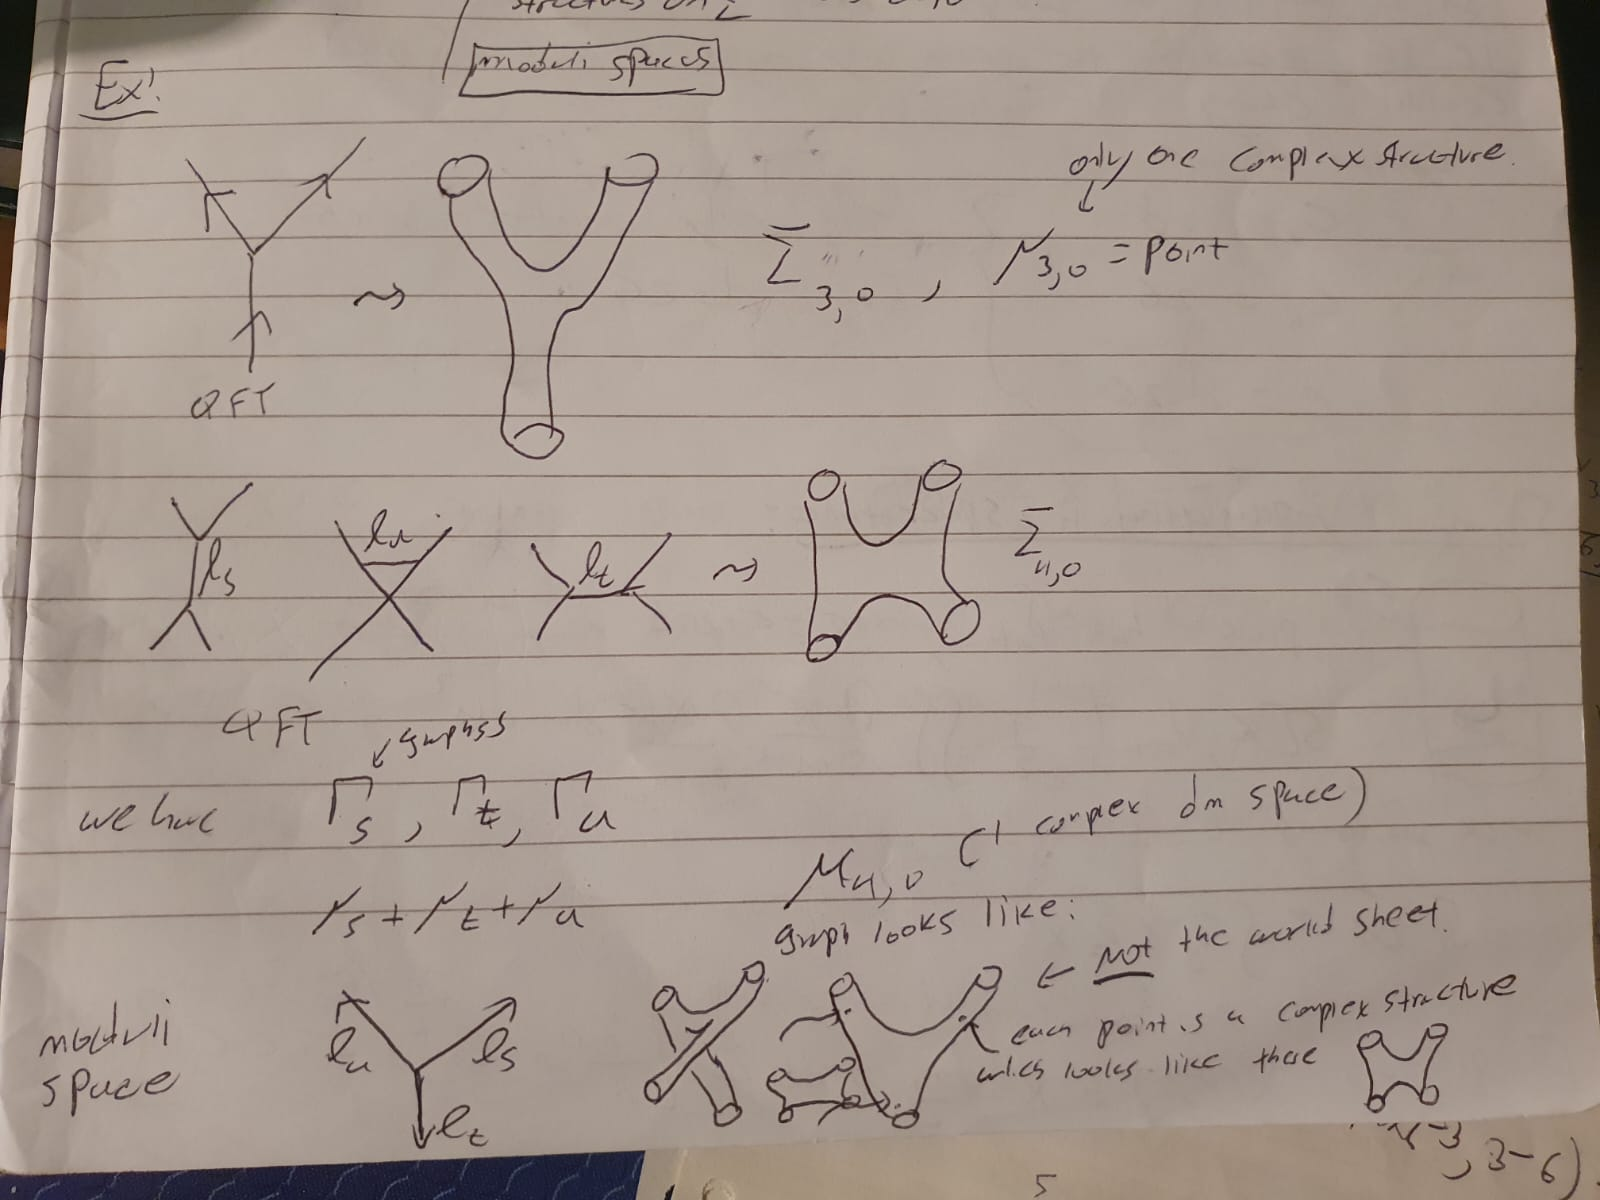
\includegraphics[scale=0.2]{moduli}
    \end{center}
   
\end{figure}

\subsection{Cohmological QFT}
Cohmological QFTs are theories with Grassman odd symmetry $Q$ ($Q^2=0$) observables are those {\bf closed} that are not exact. 
$$\text{physical obs.}=\frac{Q-\text{closed}}{Q-\text{exact}}$$
as correlations are preserved iff $Q$ acts on them. We can describe operators $X^\mu$ and $QX=C$ (secretly $dx^\mu$) as $Q$ is secretly $d$,
with $QC=0$. So $f_{\mu_1 ... \mu_n}(X) C^{\mu_1}..C^{\mu_n}$ can be integrated on 
$$\int dx_1 \dots dx_n  dC_1\dots dC_n f_{\mu_1 ... \mu_n}(X) C^{\mu_1}..C^{\mu_n} \equiv \langle f \rangle =\int f$$
so we intrinsically had to integrate over the $C$ variables to find the $f$ correlation. Studying $H(Q)$ is studying the topology
of the manifold as we study correlation function.

\subsubsection{Menaing of gohsts}
Instead of considering orbits as $1$ point, we introduce ghosts along the orbits such that locally they cancel out the bosonic directions, i.e. they reproduce the 
true degrees of freedom.

Obsercables of the form $\mathcal{O}(X,C)=\mathcal{O}_{\mu_1\dots\mu_n} C^{i_1}\dots C^{i_n}$ wich can be seen as forms by $C\to dx$, $Q \to d$, then 
$$\int_N \omega=\int_M \omega \wedge df_1 \delta(f_1) \wedge ... \wedge df_n \delta(f_n)$$
where $N_{d-1}\subset M_d$ defined by $\{f_\alpha(x)=0\}_{\alpha=1^n}$. 

One representation is 
$$df_n\delta(f_n)=\int dB^i e^{i B^i f_\alpha} \int db^\alpha e^{b^\alpha d f_\alpha}$$
so \begin{equation}
    \int dx dC dB db e^{iB^a f_a +b^a \partial_i f_a^{c^i} } \mathcal{O} \mathcal{O} \mathcal{O}
\end{equation}
still has $Q$ symmetry $$\begin{cases}
    Qb=-B i\\
    QB=0
\end{cases}$$


\begin{example}
    Consider $$\int_{\RR} \frac{\partial f}{\partial x} \delta(f(x))= \sum_{x_i, \text{s.t. }f(x_i)=0} \text{sign}( \frac{\partial f}{\partial x} )$$
    is a topological invariant. One if the graph goes from $-\infty$ to $\infty$ and $0$ if it dont.
    \begin{figure}
        \begin{center}
            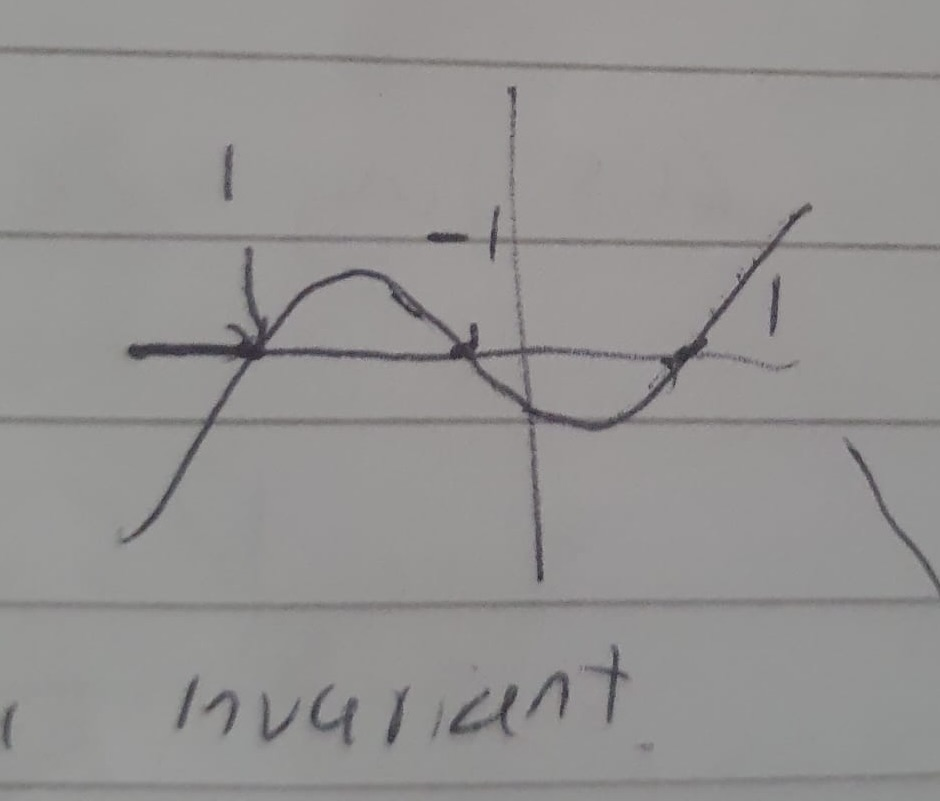
\includegraphics[scale=0.2]{topinv}
       \caption{Image of manifold with a courve in the principla bundle. One curve intersecting the orbits perpendicular is fine. 
       A curve with some topologicall twists is also fine due to the example above.}    
        \end{center}
       
    \end{figure}
\end{example}
Let $M$ be a manifold, $G$ a Lie group acting on $M$, $t^a$ generators of the lie algebra, 
\begin{align}
    QX^i=C^a v_a^i(x) \implies Q f(X)= C^a v_a^i  \frac{\partial f}{\partial x^i}\\
    Q^2X=0 =QC^a v_a^i(x) = C^a C^b \partial_j v_{[a}^j v_{b]}^i =C^a C^b \partial_j  f_{ab}^c v_c^i 
\end{align}

\begin{align}
    QC^a=f_{bc}^a C^b C^c \\
    Q^2 C^a = f^a_{[b \alpha} f^{\alpha}_{de]}C^bC^d C^e =0 \text{due to jacobi} \implies \text{self consistent}
\end{align}
so we can talk about integrals in the space of orbits. If i want to gauge fix I put a bunch of constraints 
$  \{f_\alpha(x)=0\}\to B$ then a correlation function is 
$$Z \to \int dX dc dB db e^{Qf^ab_a} \mathcal{O}_1 \dots \mathcal{O}_n$$ 
this evaluate on this constraints:
\begin{figure}
    \begin{center}
        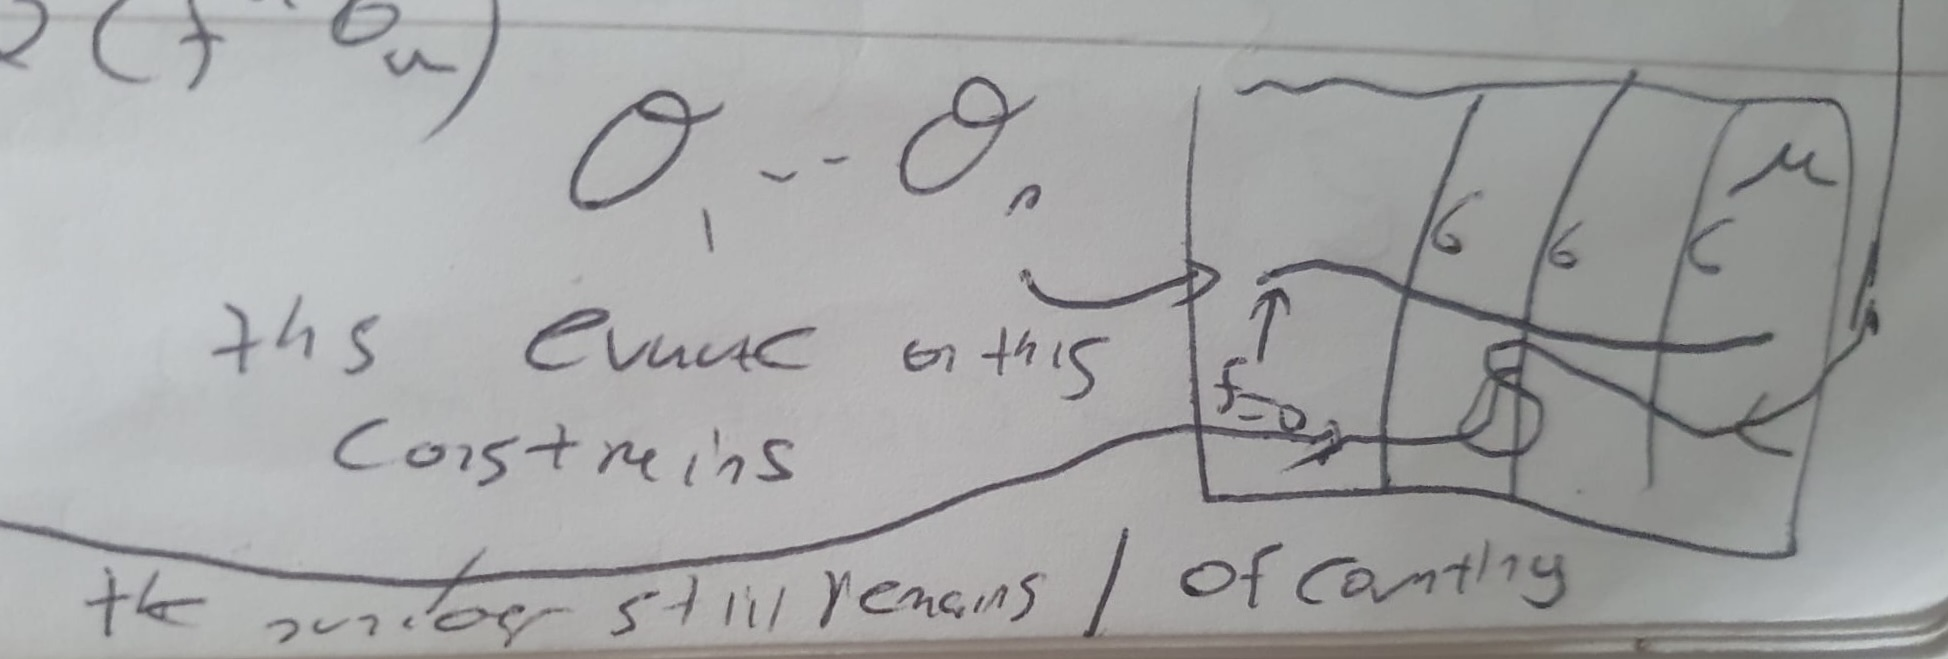
\includegraphics[scale=0.2]{sections1}
   \caption{Image of manifold with a courve in the principla bundle. One curve intersecting the orbits perpendicular is fine. 
   A curve with some topologicall twists is also fine due to the example above.}    
    \end{center}
   
\end{figure}

\begin{equation}
    \int dx dc dB db e^{Q(f^a b_a)}  \mathcal{O}_1 ... \mathcal{O}_n = \int_{\mathcal{M}/G} \implies Z= \int dx ... e^{Q(f_a b^a)+ S[x]}  \mathcal{O}_1\dots  \mathcal{O}_n = \int_{\mathcal{M}/G} e^{S[x]}  \mathcal{O}_1\dots  \mathcal{O}_n
\end{equation}
\subsection{String theory?}
If $X(t,x),$ 
\begin{equation}
    \int dx dc dc_t dt dB db e^{iB^a f_a(x,t)+ b^a \partial_i f_a(x,t) c^i +b^a \partial_t f_a(x,t) c^t} \mathcal{O}_1 ... \mathcal{O}_n 
\end{equation}
we always locally gauge fix to be flat the metric using Weyl symmetry but we cannot globally. 
\begin{equation}
    \int D X^\mu D h^{ab} D c^a D c_{\text{Weyl}} Db^{ab} DB^{ab} \underbrace{d \mu}_{(1)} \underbrace{dC_\mu}_{(2)}
\end{equation}
where $(1)=$ possible states of complex structures (finite dimensional) and $(2)$ partners. Note $C^a$ are functions on the surface $\Sigma$ to the tangent bundle.
$$QX^\mu =C^a \nabla_a X^\mu,\quad Q h_{ab}= \nabla_a C_b \nabla_b C_a +h_{ab} C^{Weyl}, \quad Q b^{ab}=B^{ab}$$
$$\quad QC^{\text{Weyl}}=C^a \partial_a C^{Weyl}, \quad QC^a =C^b \nabla_b C^a$$
s
o $Q(b^{ab}(h_{ab}-\hat{h}_{ab}(\mu)))=B^{ab}(h_{ab}-\hat{h}_{ab}(\mu))-b^{ab}(\nabla_a c_b +\nabla_b c_a)-b^{ab}(h_{ab}C^{Weyl}) +b^{ab} \frac{\partial \hat{h}_{ab}}{\partial \mu} \hat{C}^\mu$

Now, integrate out $B,h,b^{ab},h_{ab},C^{Weyl},\hat{C}^\mu$ 
\begin{equation}
    \int \mathcal{D}X D b^{ab} D C^a e^{S[X,\hat{h}_{ab}(\mu)]+S_{gf}[\hat{h}_{ab}(\mu)]} \prod b^{ab} \frac{\partial \hat{h}_{ab}}{\partial \mu^i} \underbrace{d\mu^i}_{\text{Cplx. stru.}}
\end{equation}
Where the $X$ integral computes the correlation function of some field theory. {\bf Caution!} When you integrate out fields 
you replace them with the EOM so for $h$ we have a contribution from the action $S_X$ and from $Q(b^{ab}(h_ab-\hat{h}_{ab}))$ i.e. 
the term $B^{ab}(h_{ab}-\hat{h}_{ab}(M))$. This sets $$\frac{\delta S}{\delta h_{ab}}= B^{ab}=T^{ab}$$

\begin{example}
    In the finite case,
    $$\int dxdc dB db e^{\underbrace{iB^a f_a (x)+ b^a \partial_i f_a c^i +B^2}_{-Q(b^a f_a +b B)}}= \int dx dc db e^{-f^2 +b^a \partial_i f_a c^i}$$
    as $B$ is exact. but now the transformation of $b$ i.e. $Qb=f$  but $Q^2 b= \partial_i f c^i$ this only vanishes because equation of motion 
    set $\partial_i f=0$ but not identically.
\end{example}

CFT of the Ghost and so on\dots $J_{gh}=bc$ 
$$\{Q,b\}=T =T_X+T_{gh}$$
$$T_{gh}=c \partial b +2 \partial c b, \quad J_{BRST}=cT_x +bc \partial c \implies Q=\int J_{BRST}+ \bar{J}_{BRST}$$

$$\{Q,b_n\}=L_n$$

$Q^2 \sim (d-26)$

Physical states:

$$L_n \ket{n} \otimes \ket{0}=\{Q,b_n\}\ket{n} \otimes \ket{0} = 0 $$
so physical states are those in cohmology. It is sufficient as $\ket{\tilde{m}}=L_n \ket{m}$, $m<0$ reduces to 
\begin{align}
    Q (b_n \ket{\tilde{m}} \otimes \ket{0})= L_n \ket{\tilde{m}} \otimes \ket{0}+ b_n Q \ket{\tilde{m}} \otimes \ket{0}=...= L_n \ket{\tilde{m}} \otimes \ket{0}
\end{align}
So physical states are indeed in BRST cohmology.


\section{Complex structures}
Stereographic projection of the plane to the sphere. Plane to cylinder gives$z=e^s$,
$$\frac{dz d\bar{z}}{|z|^2}=ds d\bar{s}$$
and sphere to cilinder $$\frac{ds d\bar{s}}{(e^{(s+\bar{s})/2}+e^{-(s+\bar{s})/2})^2}.$$


What if we take  plane with three marked points (punctured) $$dz d\bar{z}(1+ \frac{1}{|z-z_1|^2}+\frac{1}{|z-z_2|^2}+\frac{1}{|z-z_3|^2} )$$
and, if I remove one point the topology is that of a 3 punctured sphere.
In general 
\begin{equation}
    dz d\bar{z}(\sum_{ij} \frac{1}{|z-z_i|^2 |z-z_j|^2}¡ )
\end{equation}

In general, if you start from a $n$ punctured sphere, diffeomorphism that map the metric to itself? rotations.
But what about complex structures allowed? We already chose that by taking $z$ coordinates so we can find $z=z(z')$ global 
a diffeo i.e. that maps the punctured sphere to a punctured sphere in other places. For this we set $z=\frac{az'+b}{cz'+d}$ this work fine in 
the sphere (only dosent work in infinity as it sends to 1 points) we can take $ad-bc=1$  which then defines an $PSL(2,\CC)$ action. 

\begin{example}
    $SL(2,\CC)$ $z\to \lambda z$ (rescaling) so these are rescaling, rotations (if $\lambda$ is aphase), etc. These are the transf 
    that lives the metric conformally flat. If we take a generic function $z=f(z')$ it dosent map to the sphere to sphere $1-1$, $Mobius$ transformation 
    are special in this sense. Maps are really sensitive to holomorphy to not have poles and behave well.

    For example, suppose there is an invertible map from plane to sphere (which can't be among other reasons because $S^2$ is compact) this is equivalent 
    to say to find a function on the sphere holomorphic and with no poles. Using Liouville's theorem, this function is bounded 
    and holomorphic $\implies$ constant function $\implies$ non invertible.
\end{example}

Vector fields on the sphre that are globally well defined and holo are $\{\partial, z \partial , z^2 \partial\}$ and their respective 
conjugates. This Mobius transform moves three points:
$z'=\frac{z-z_1}{z-z_3} \frac{z_2-z_3}{z_2-z_1}$ this gives $z_2 \to 1$ $z_1 \to 0$ $z_3 \to \infty$.
\begin{figure}
    \begin{center}
        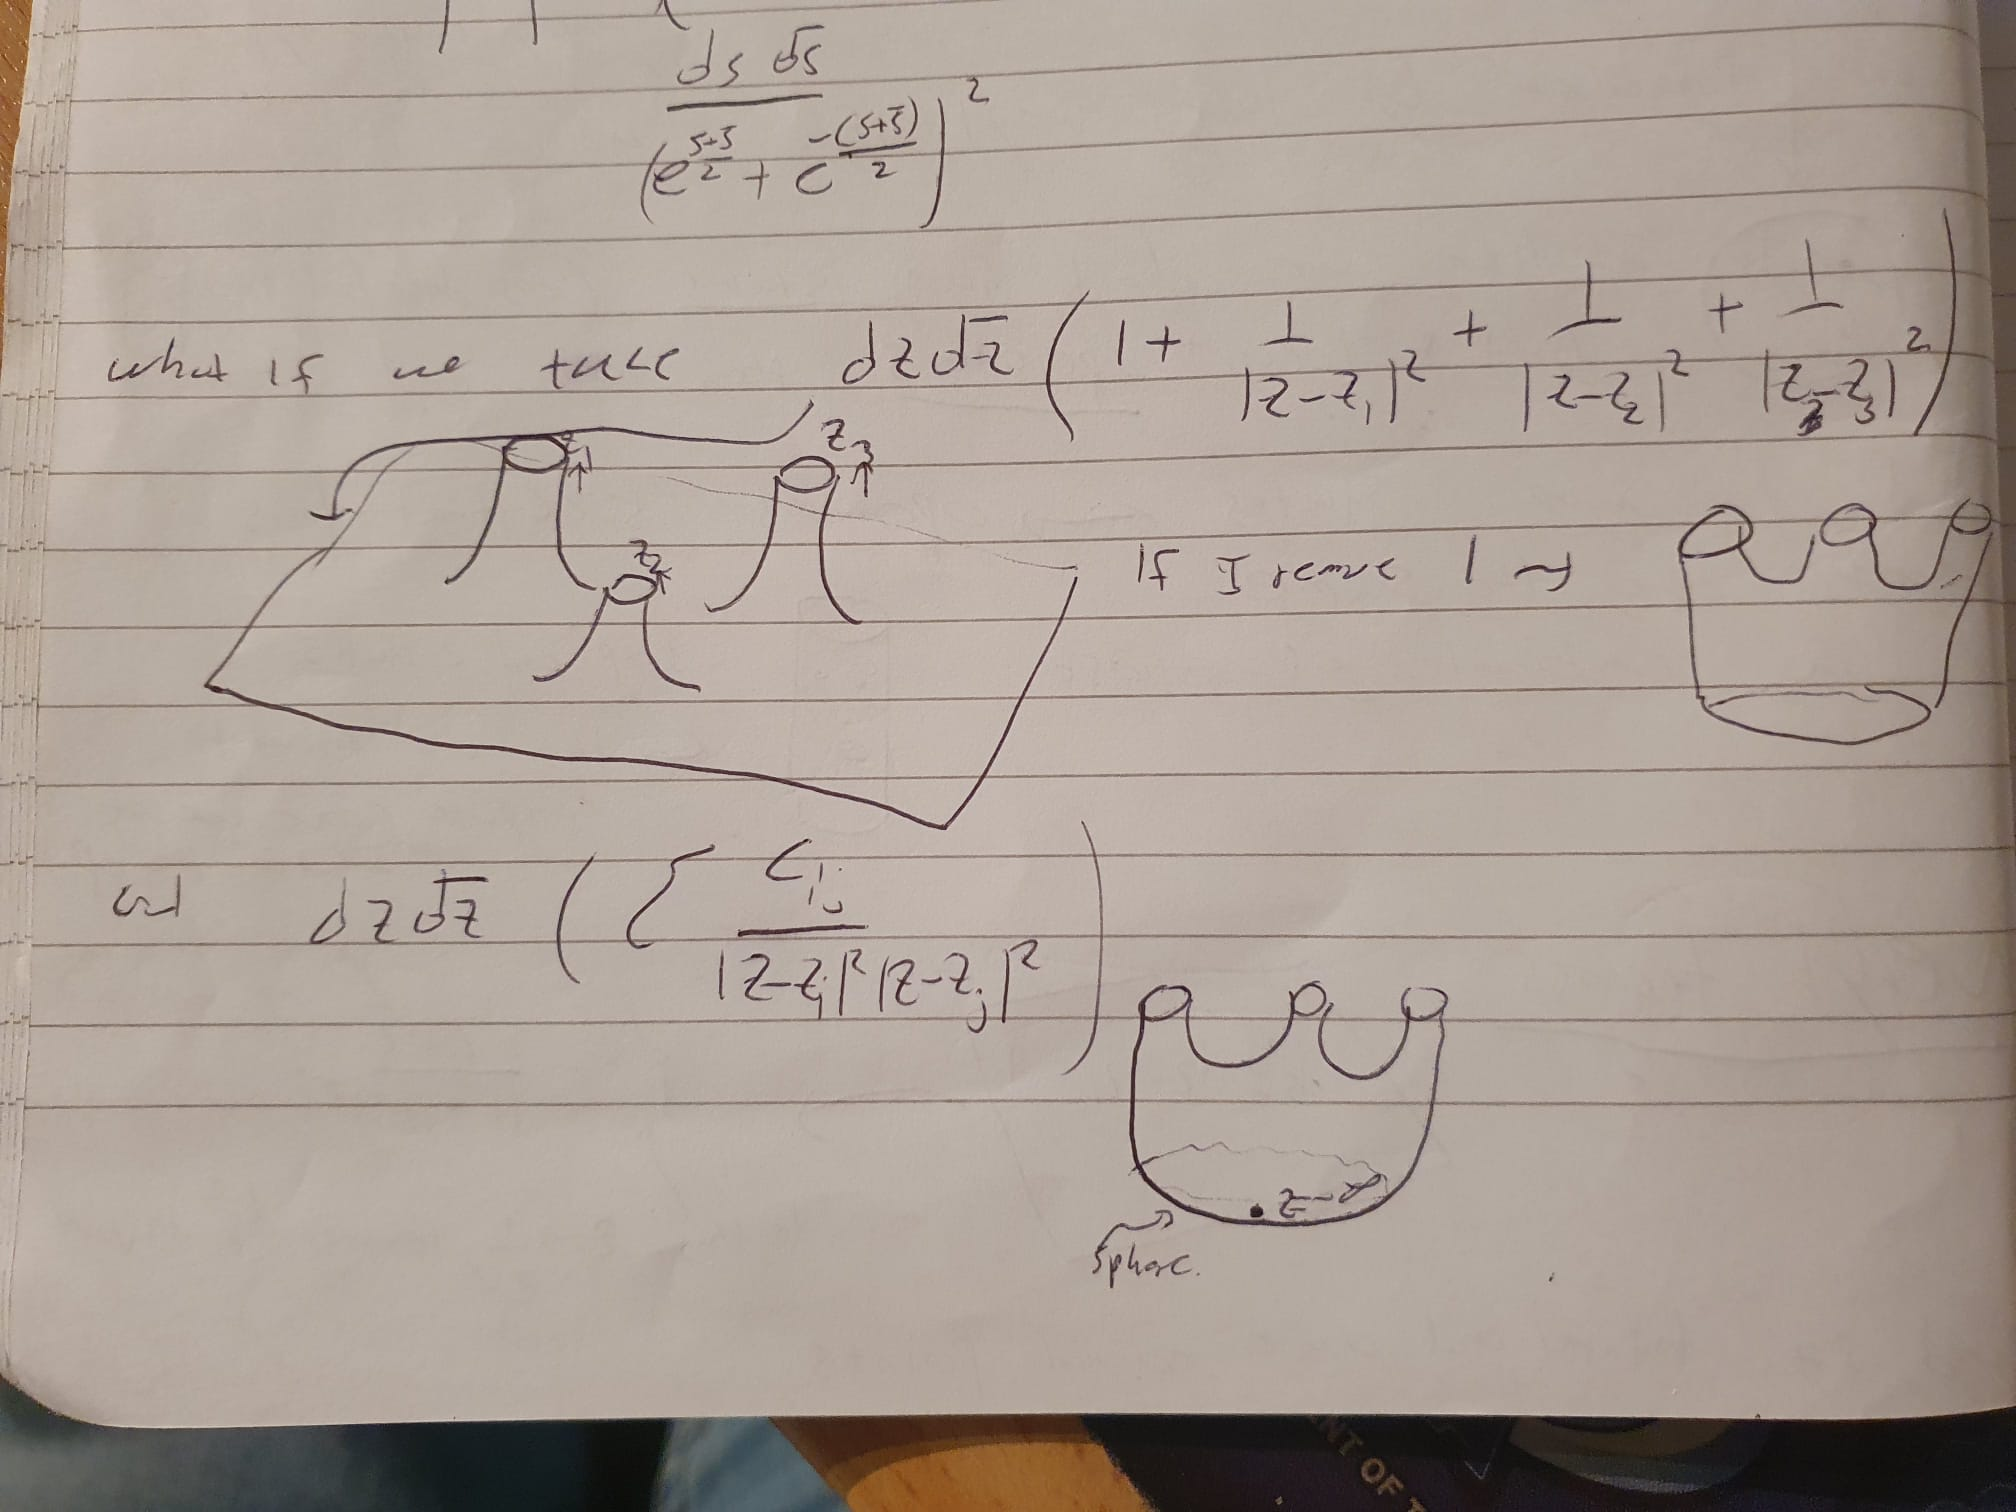
\includegraphics[scale=0.2]{complexs}
    \end{center}
\end{figure}
For $4$-pt functions the best is $z_2 \to 1$ $z_1 \to 0$ $z_3 \to \infty$ and $z_4 \to z_4'$. $$z'=\frac{z-z_1}{z-z_3}\frac{z_2-z_3}{z_2-z_1}$$
so for $3$ points we can always map in the above way, no freedom. For $4$ points we have $1$ freedom. 

Hence, $$\mathcal{M}_{0,3}= \{\cdot\}$$
$$\mathcal{M}_{0,4}=S^2-\{0,1,\infty\}$$
\begin{figure}
    \begin{center}
        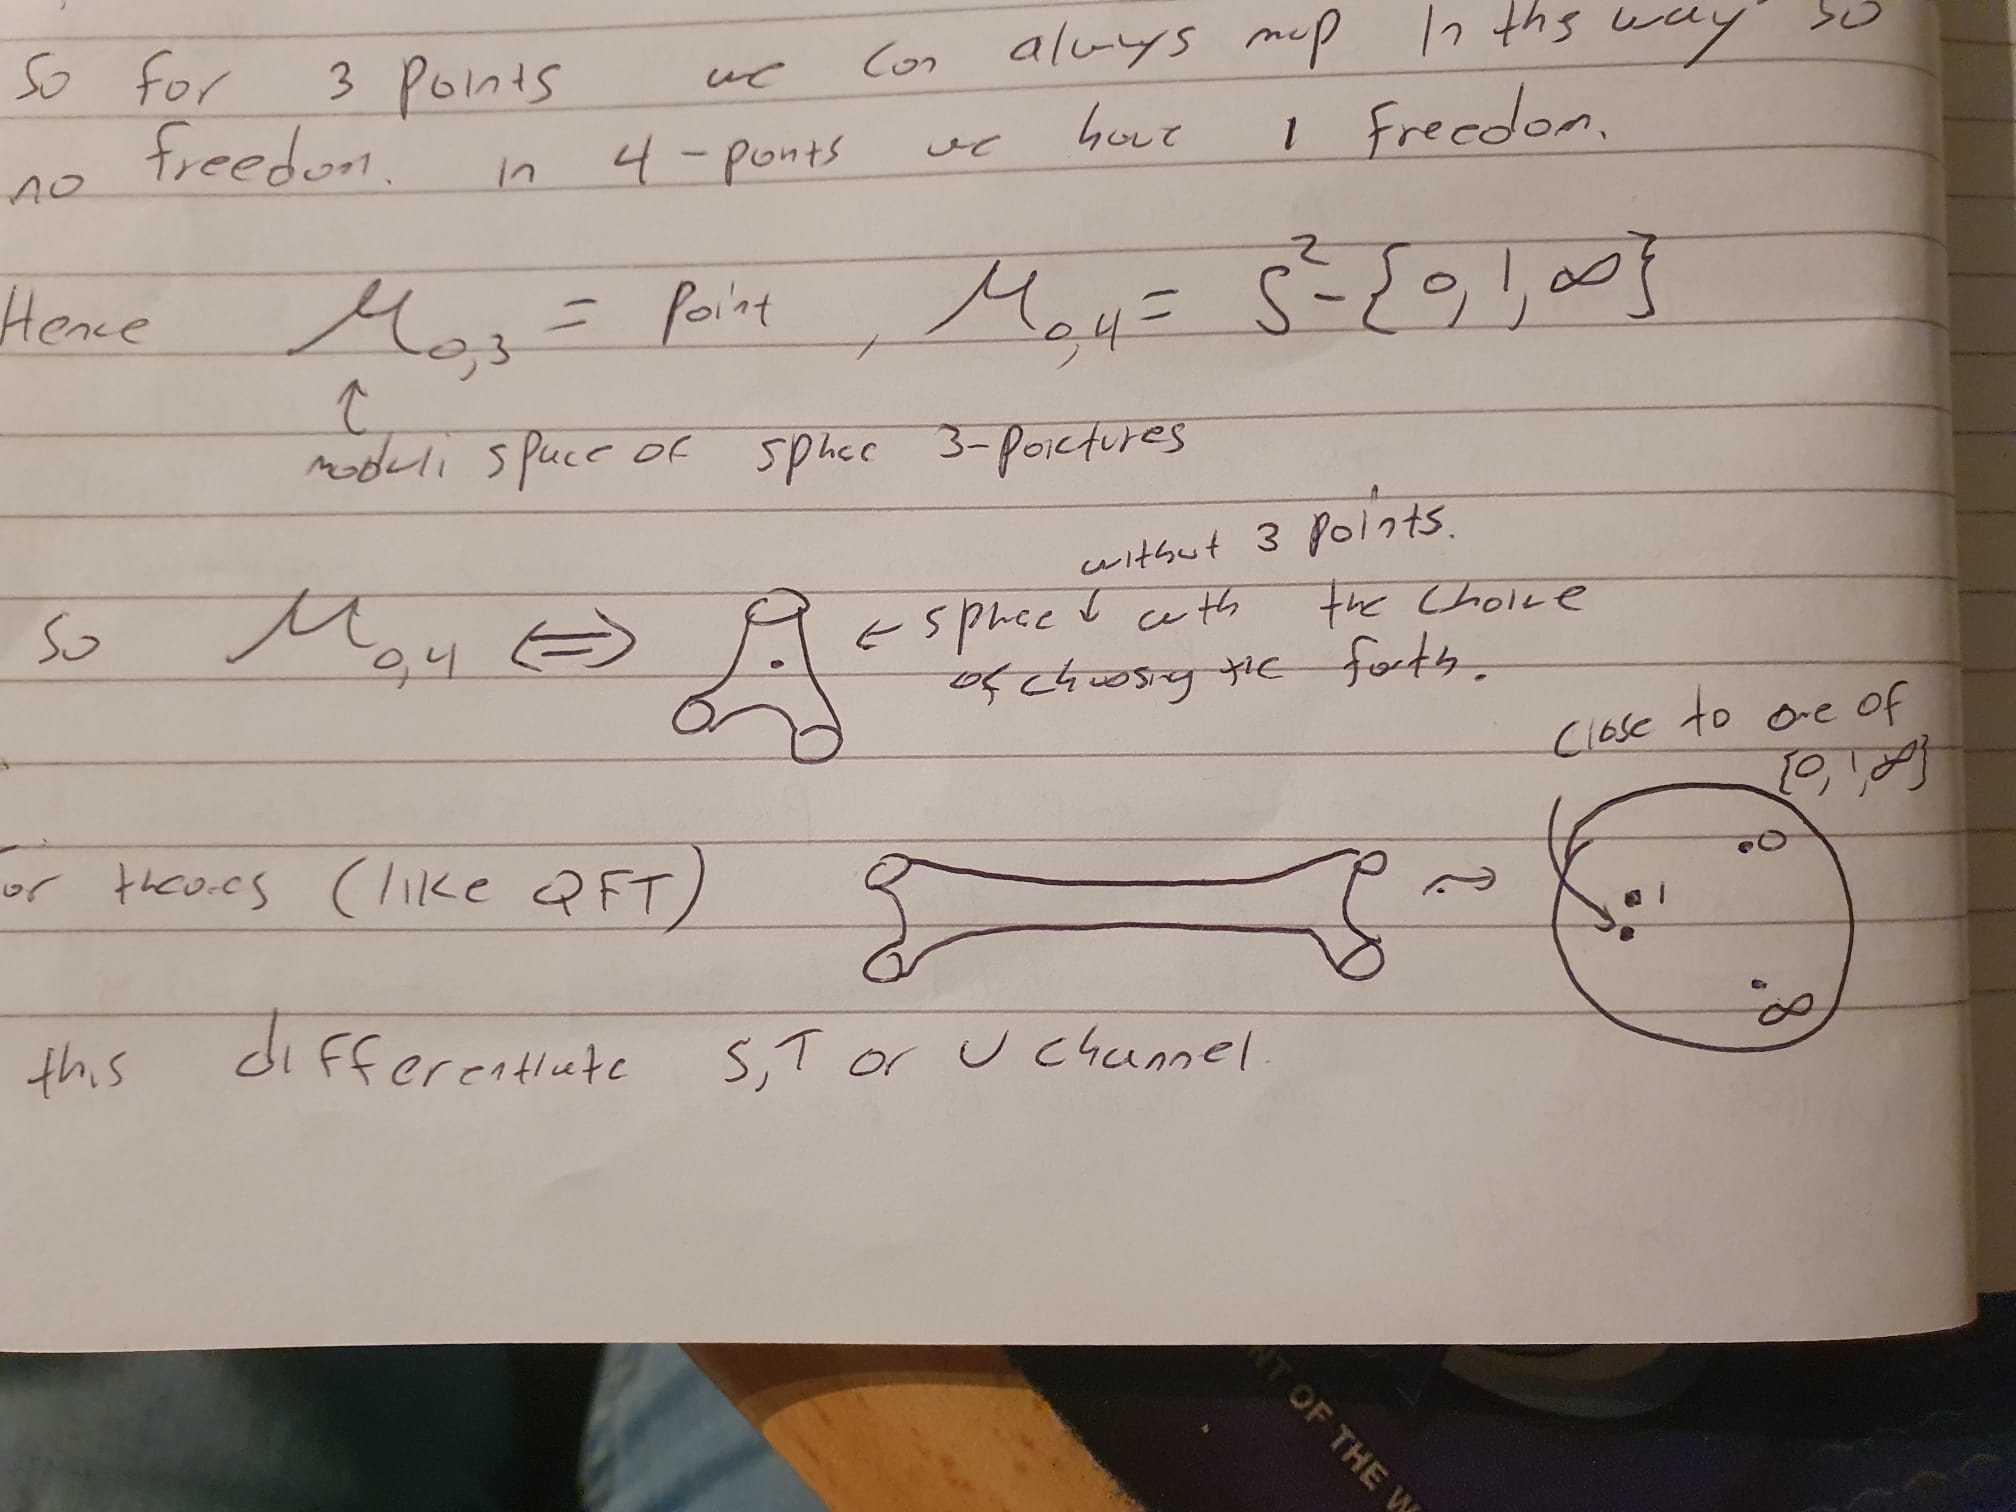
\includegraphics[scale=0.2]{moduli3}
    \end{center}
\end{figure}
so $\mathcal{M}_{0,4}$ is a "pair of pants" = sphere with 3 distinguished points.

For theories like QFT, the different $s,t$ and $u$ channels. So moduli is just a line.




\section{The Moore-Seiberg Construction on RCFTs}

\section{Modular bootstrap and line defects}





\end{document}
